\subsection{SET: Comparison to ``symbolic'' model}
In~\Cref{fig:exp_set_symbolic}, we compare an Abstractor-based model to a ``symbolic'' model which receives as input a binary representation of the four relevant relations. The same CNN embedder as in the previous SET experiment is used. Next, we train 1-head Abstractors separately for each of the four attributes to learn same/different relations, where the task is to decide if an input pair of cards is the same or different for that attribute. We then use the learned $W_1$ and $W_2$ parameters learned for these relations to initialize the relations in a multi-head Abstractor. The Abstractor is then trained on a dataset of triples of cards, half of which form a SET.

This is compared to a baseline symbolic model where, instead of images, the input is a vector with 12 bits,
explicitly encoding the relations. That is, for each of the four attributes, a binary symbol is computed for each pair of three input cards---1 if the pair is the same in that attribute, and 0 otherwise. A two-layer MLP is then trained to decide if the triple forms a SET. The MLP using the symbolic representation represents an upper bound on the performance achievable by any model. This comparison shows that the Abstractor is able to solve a task using relations learned in other tasks (modularity), with a sample efficiency that is not far from that obtained with purely symbolic, noise-free encodings of the relevant relations.

\begin{figure}[ht]
    \centering

    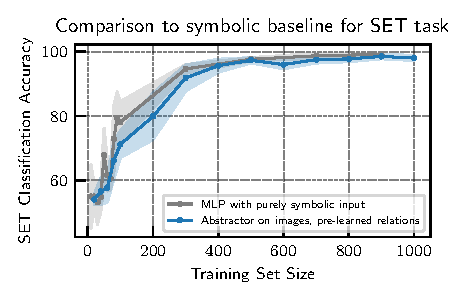
\includegraphics{figures/experiments/set_symbolic_vs_abstractor.pdf}
    \caption{Comparison of Abstractor trained card images and MLP with hand-encoded relations.}% The Abstractor is nearly as sample 
    \label{fig:exp_set_symbolic}
\end{figure}